\section{HA 08: Beschreibung Kaufprozess Elektronikkauf}
  Bevor neue Elektronikgeräte gekauft werden, sollte man sich besonders lange mit der Frage beschäftigen: "Brauche ich das wirklich?" Der Aufwand an Ressourcen und Energie zur Herstellung des Produktes steht oft in keinem Verhältnis zu der sinnvollen Anwendung. Oft stehen die Geräte nach zweimaliger Benutzung im Schrank und dienen nur als Deko. Erst wenn das Gerät wirklich akut benötigt wird, sollte man meiner Meinung nach über einen Kauf nachdenken. In der schematischen Darstellung beginnt der Kaufprozess daher mit der Situation, in der ein bestimmtes Gerät benötigt wird.\\\\
  Ist die Situation eingetreten, bei der die gewünschte Elektronik wirklich benötigt wird, lässt sie sich in vielen Fällen leihen oder mieten. Eine weitere Alternative ist der Gebrauchtkauf, bei der weniger Geld ausgegeben und nachhaltiger gehandelt wird.\\\\
  Tritt wiederholt der Fall ein, dass das Gerät gebraucht wird und Mieten und Gebrauchtkauf nicht in Frage kommen, sollte man sich über das Angebot der unterschiedlichen Anbieter eingehend informieren um einen Fehlkauf zu vermeiden. Ist dann teils aus dem Bauchgefühl und teils auf einer subjektiven Entscheidung heraus das passende Gerät gefunden, kann noch nach Vergünstigungen und in unterschiedlichen Läden, online wie offline, gesucht werden um das perfekte Angebot zu finden.\\
  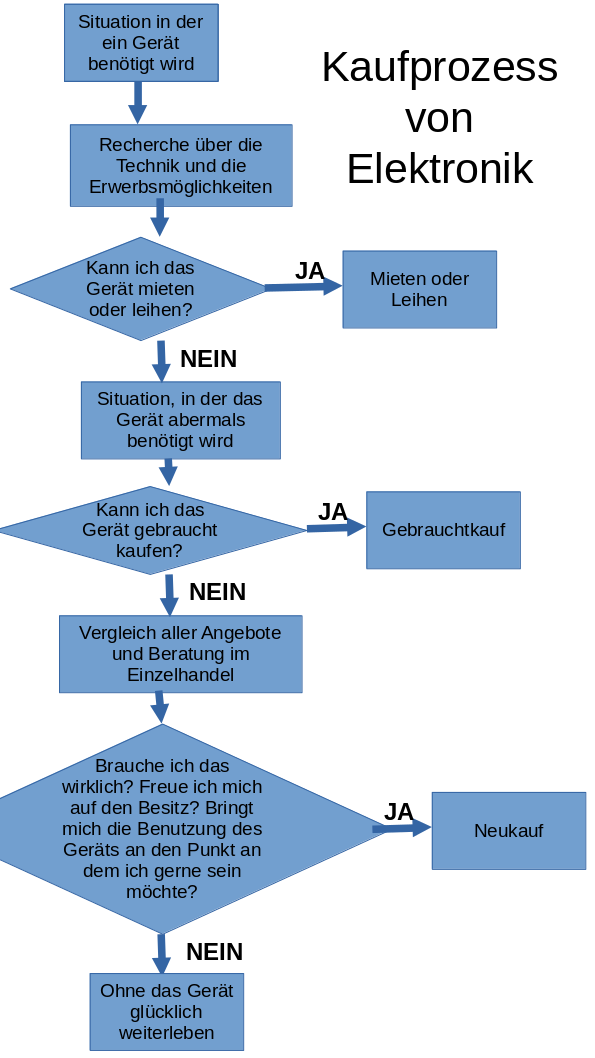
\includegraphics[scale=0.6]{Hausaufgaben/8_Kaufprozess/Kaufprozess_Grafik.png}
